%% This is an example first chapter.  You should put chapter/appendix that you
%% write into a separate file, and add a line \include{yourfilename} to
%% main.tex, where `yourfilename.tex' is the name of the chapter/appendix file.
%% You can process specific files by typing their names in at the 
%% \files=
%% prompt when you run the file main.tex through LaTeX.
\chapter{Introduction}

Many systems must support concurrent access by hundreds or thousands of users. Failure to providing scalable access to users may results in catastrophic failures and unfavorable media coverage \cite{Jiang2010}. 

The explosive growth of the Internet has contributed to the increased need for applications that perform at an appropriate speed. Performance problems are often detected late in the application life cycle, and the later they are discovered, the greater the cost to fix them \cite{Molyneaux2009}.

The use of stress testing is an increasingly common practice owing to the increasing number of users. In this scenario, the inadequate treatment of a workload generated by concurrent or simultaneous access due to several users can result in highly critical failures and negatively affect the customers perception of the company \cite{Draheim2006b} \cite{Jiang2010}. 

Stress testing determines the responsiveness, throughput, reliability, or scalability of a system under a given workload. The quality of the results of applying a given load testing to a system is closely linked to the implementation of the workload strategy. The performance of many applications depends on the load applied under different conditions. In some cases, performance degradation and failures arise only in stress conditions \cite{Garousi2010} \cite{Jiang2010}.


A stress test uses a set of workloads that consist of many types of usage scenarios and a combination of different numbers of users. A load is typically based on an operational profile. Different parts of an application should be tested under various parameters and stress conditions \cite{Babbar2011}. The correct application of a stress test should cover most parts of an application above the expected load conditions\cite{Draheim2006b}.


Fig. \ref{fig:example} shows an example of a system under assessment with three pages (the main page, profile page, and search page) and six possible users. From the combinations of users and application pages, various scenarios can be created, such as scenarios 1 and 2 shown in the figure. The first scenario presents a test that has passed, and the second scenario presents a test that has an HTTP 404 error.

\begin{figure}[ht]
\centering
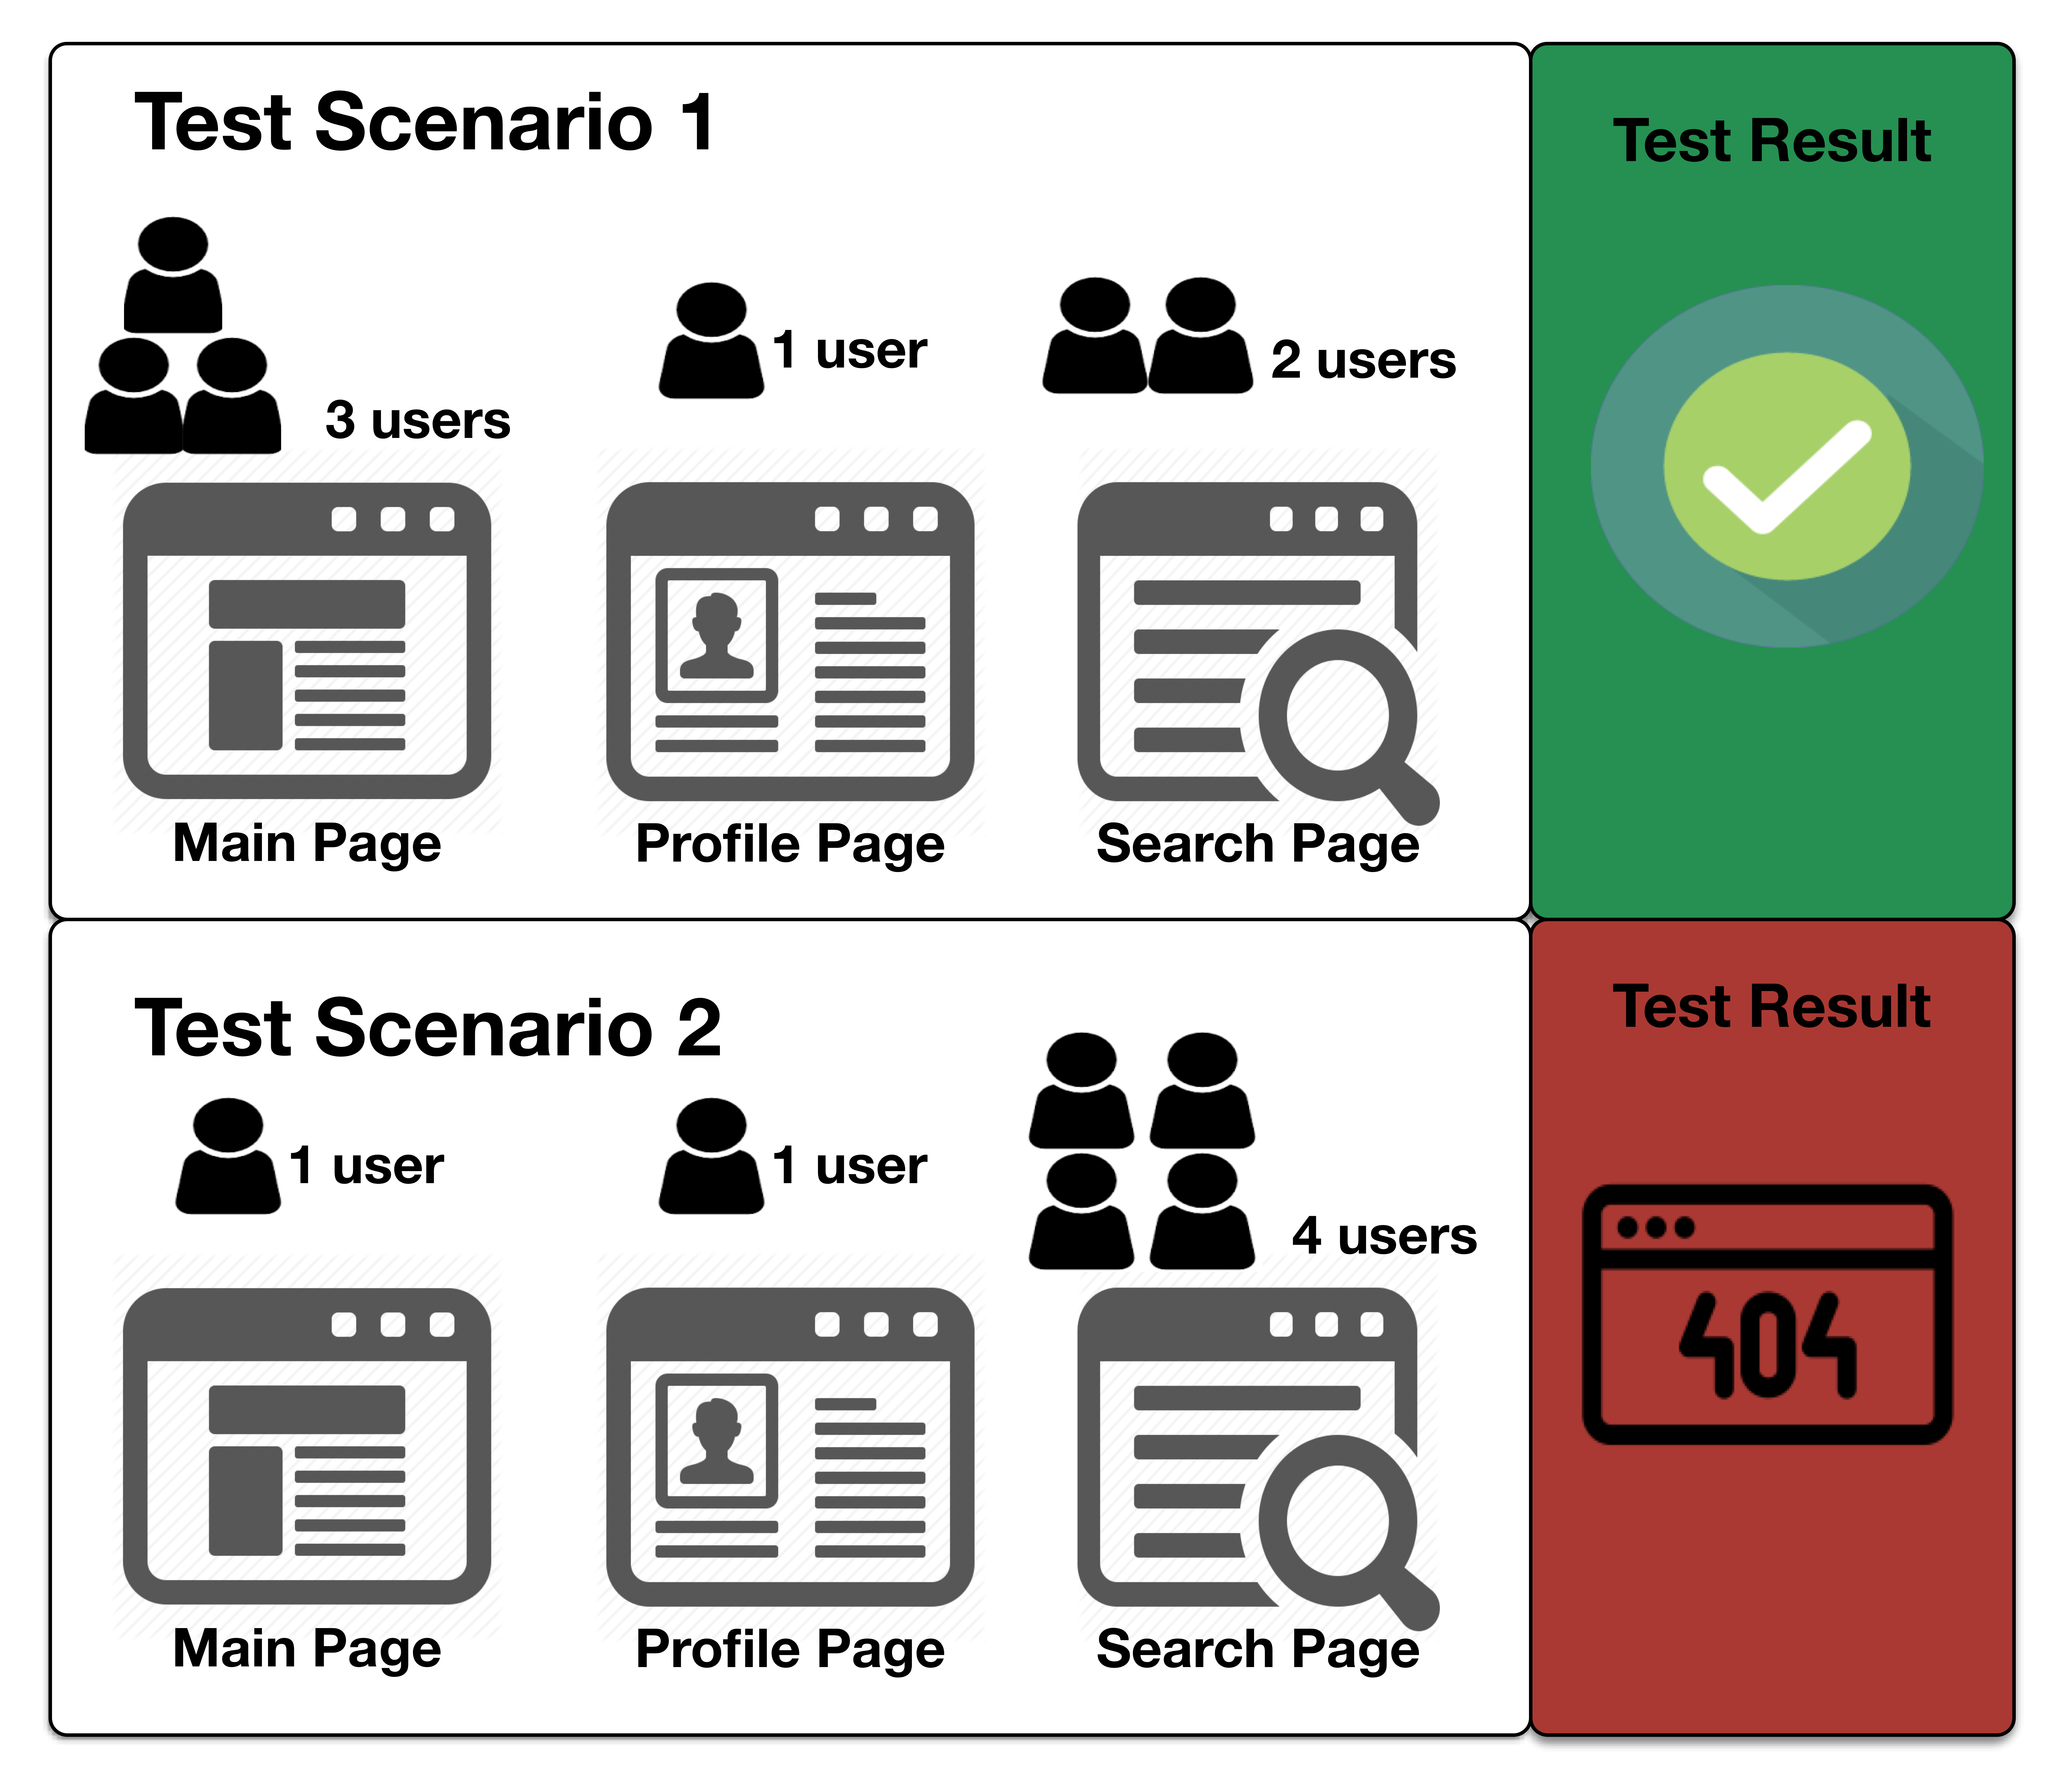
\includegraphics[width=0.4\textwidth]{./images/diagram.png}
\caption{Possible test scenarios for a hypothetical application}
\label{fig:example}
\end{figure}

A stress test usually lasts for several hours or even a few days and only tests a limited number of workloads. The major challenge is to find the workloads that expose a major number of errors and to discover the maximum number of users supported by an application under testing \cite{Barna2011}. 

Search-based testing is seen as a promising approach to verifying timing constraints \cite{Afzal2009a}. A common objective of a load search-based test is to find  scenarios that produce execution times that violate the specified timing constraints \cite{Sullivan}. 

This paper has two main goals:

\begin{itemize}
\item  To ascertain whether hybrid algorithms are superior to single metaheuristics when solving stress testing problem.
\item To improve the process of stress testing with a tool and a test model that evolves during its execution.
\end{itemize}


\begin{figure}[ht]
\centering
\includegraphics[width=0.25\textwidth]{./images/solution.png}
\caption{Illustrative example showing how IAdapter should be used}
\label{fig:solution}
\end{figure}


This paper proposes the use of a hybrid metaheuristic approach that combines genetic algorithms, simulated annealing, and tabu search algorithms in stress tests. A tool named IAdapter (www.iadapter.org, github.com/naubergois/newiadapter), a JMeter plugin for performing search-based load tests, was developed. Two experiments were conducted to validate the proposed approach. The first experiment was performed on an emulated component, and the second one was performed using an installed Moodle application.

Fig. \ref{fig:solution} shows an example where IAdapter stress test automation finds two test scenarios. The first scenario presents a test that has an HTTP 500 error, and the second scenario presents a test that has a response time higher than 30 seconds. 


\section{Motivation}

Software testing is a expensive and difficult activity. The exponential
growth in the complexity of software makes the cost of testing has only continued to rise. Test case generation can be seen as a search problem. The test adequacy criterion is transformed into a fitness function and a set of solutions in the search
space are evaluated with respect to the fitness function using a metaheuristic search technique. Search-based software testing is the application of metaheuristic search techniques to generate software
tests cases or perform test execution \cite{Afzal2009a} \cite{Gay}.

Experimentation is important to realistically and accurately test and evaluate search based tests. Experimentation on algorithms is usually made by simulation. Experiments involving search based tests are inherently complex and typically time-consuming to set up and execute. Such experiments are also extremely difficult to repeat. People who might want to duplicate published results, for example, must devote substantial resources to setting up and the environmental conditions are likely to be substantially different.




\section{State of Research on the Search-Based Stress  Testing}

In the academic context, a number of studies proving the efficacy of metaheuristics to automate test execution can be found in literature \cite{Afzal2009a}. 

\section{State of Industrial Practices on Stress Tests}

The stress testing process in the industry still follows a non-automated and ad-hoc model where the designer or tester is responsible for running the tests analyzing the results and deciding which new tests should be performed \cite{Lewis2005}. Current approaches to load testing suffer from limitations. Their cost-effectiveness is highly dependent on the particular test scenarios that are used yet there is no support for choosing those scenarios. A poor choice of scenarios could lead to underestimating system response time thereby missing an opportunity to detect a performance fault \cite{Zhang2011}.


\section{Research Hypothesis}





Our underlying research hypothesis is as follows:

\begin{mybox}
The use of metaheuristics and hybrid metaheuristics in combination with Q-learning can make it possible to automate the stress test execution process, improving the choice of new test cases for each interaction and finding scenarios that maximize the number of users of the application under test and minimize response time or find scenarios with a expected response time.
\end{mybox}

The purpose of this thesis is to show the validity of this hypothesis through the development of a testbed tool, algorithms that use hybrid metaheuristics and the Q-learning technique and application of validation experiments. This thesis will be useful for load test practitioners and software engineering researchers interested in large-scale testing software systems.


\section{Thesis Overview}

In this section, we present an overview of the works presented in this thesis. This thesis has five main chapters

\section{Thesis Contributions}

The major contributions of this thesis are:

\begin{itemize}
\item Hybrid Metaheuristic Approach \cite{Gois2016}: 
\item Q-Learning Metaheuristic Approach: 
\item IAdapter JMeter Plugin:
\item Testbed Tool: 
\end{itemize}




\section{Thesis Organization}


